% IEEE conference paper: SVM-based transient stability assessment of the IEEE 39-bus system.
% Compile with pdflatex (run twice). Figures are read from ./figures/ (make_paper_figures.py).
\documentclass[conference]{IEEEtran}
\IEEEoverridecommandlockouts
\usepackage{cite}
\usepackage{amsmath,amssymb,amsfonts}
\usepackage{graphicx}
\usepackage{textcomp}
\usepackage{xcolor}
\usepackage{booktabs}
\usepackage{tikz}
\usetikzlibrary{positioning,arrows.meta}
\graphicspath{{figures/}}

\begin{document}

\title{Transient Stability Assessment of the IEEE 39-Bus System Using Support Vector Machines on Post-Disturbance
Generator Voltage and Frequency Samples}

% TODO: replace the placeholders with the author names and affiliations
\author{\IEEEauthorblockN{First Author}
\IEEEauthorblockA{\textit{Department of Electrical Engineering} \\
\textit{University Name}\\
City, Country \\
email address}
\and
\IEEEauthorblockN{Second Author}
\IEEEauthorblockA{\textit{Department of Electrical Engineering} \\
\textit{University Name}\\
City, Country \\
email address}
}

\maketitle

\begin{abstract}
Fast and reliable transient stability assessment (TSA) is essential for secure power-system operation. This paper
investigates a support vector machine (SVM) classifier that predicts the transient stability status of the IEEE
39-bus system from only four post-disturbance samples of the voltage magnitude and the frequency at each of the ten
generator buses. A dataset of 3\,715 time-domain simulations is used, covering generator trips, line trips,
single-line-to-ground, double-line-to-ground and three-phase-to-ground faults with line tripping, and load
disconnections at five loading levels, labelled with the transient stability index (TSI). To avoid optimistic
estimates, the data are split by contingency so that no scenario appears in more than one subset, and the
hyperparameters are selected by contingency-grouped five-fold cross-validation. The selected radial-basis-function
SVM with robust feature scaling reaches a cross-validated balanced accuracy of 0.974 and, on an unseen test set, a
balanced accuracy of 0.955 with 95.9\,\% of the unstable cases detected and an area under the ROC curve of 0.992.
The remaining errors concentrate in a few contingencies; the most systematic one arises from inputs outside the
range covered by the training data.
\end{abstract}

\begin{IEEEkeywords}
Transient stability assessment, support vector machine, machine learning, IEEE 39-bus system, transient stability
index, data leakage.
\end{IEEEkeywords}

%=====================================================================
\section{Introduction}
%=====================================================================
Transient stability is the ability of a power system to maintain synchronism when subjected to a severe disturbance
such as a short circuit or the loss of a transmission line or generator~\cite{kundur2004definition,kundur1994}.
Time-domain simulation gives an accurate verdict but is computationally demanding when many contingencies and
operating conditions must be screened in real time. The spread of phasor measurement units has therefore motivated
data-driven TSA, in which a classifier trained offline on simulated cases predicts the stability status from a
few post-disturbance measurements within milliseconds.

Support vector machines~\cite{cortes1995,scholkopf2002} are well suited to this task because they handle
high-dimensional, correlated inputs and non-linear class boundaries with few hyperparameters. They have been applied
to TSA of large systems~\cite{moulin2004} and to post-fault stability prediction from synchronized
measurements~\cite{gomez2011}. A frequent weakness of scenario-based studies, however, is the evaluation protocol:
when every contingency is simulated at several operating points and the cases are split at random, near-identical
variants of the same contingency appear in both the training and the test data, and the reported accuracy
overstates the performance on genuinely new contingencies.

The contributions of this paper are:
\begin{itemize}
  \item a TSA dataset for the IEEE 39-bus system with four contingency families, five loading levels and three
        fault clearing times, using only 80 generator-bus voltage and frequency samples as inputs;
  \item a leakage-free evaluation protocol in which the data are split by contingency and the hyperparameters are
        selected by contingency-grouped cross-validation;
  \item an RBF-kernel SVM with robust scaling, evaluated once on an untouched test set;
  \item an error and feature-importance analysis that identifies out-of-range inputs as the main systematic
        failure mode.
\end{itemize}

Section~\ref{sec:data} describes the dataset, Section~\ref{sec:method} the methodology, Section~\ref{sec:results}
the results, Section~\ref{sec:discussion} discusses them and Section~\ref{sec:conclusion} concludes.

%=====================================================================
\section{Dataset}
\label{sec:data}
%=====================================================================
\subsection{Test System and Scenarios}
The IEEE 39-bus (New England) system~\cite{athay1979} with ten generators at buses 30--39 was simulated in the time
domain. % TODO: name the simulation tool
Four contingency families were considered (Table~\ref{tab:scenarios}). Every contingency was simulated at five
operating conditions with the system load scaled by $-4$, $-2$, 0, $+2$ and $+4$\,\%. Ground faults were applied at
20\,\% and 80\,\% of the length of each of the 34 transmission lines, as single-line-to-ground (SLG),
double-line-to-ground (LLG) or three-phase-to-ground (3PHG) faults, and were cleared after 0.1, 0.3 or 0.5\,s by
tripping the line; line trips use the same three clearing times.

\begin{table}[t]
\caption{Simulated contingencies (each at five load levels)}
\label{tab:scenarios}
\centering
\begin{tabular}{lrrr}
\toprule
Contingency family & Contingencies & Cases & Unstable (\%) \\
\midrule
Generator trip            & 10  & 50     & 10.0 \\
Ground fault + line trip  & 612 & 3\,060 & 15.0 \\
\quad SLG                 & 204 & 1\,020 & 2.9 \\
\quad LLG                 & 204 & 1\,020 & 7.1 \\
\quad 3PHG                & 204 & 1\,020 & 34.9 \\
Line trip                 & 102 & 510    & 41.8 \\
Load disconnection        & 19  & 95     & 0.0 \\
\midrule
Total                     & 743 & 3\,715 & 18.2 \\
\bottomrule
\end{tabular}
\end{table}

\subsection{Inputs and Stability Label}
For each generator bus B30--B39, four post-disturbance samples of the voltage magnitude (p.u.) and four samples of
the frequency (Hz) are recorded, giving $10 \times (4+4) = 80$ inputs. % TODO: state the sampling instants
The label is obtained from the transient stability index~\cite{xu2012}
\begin{equation}
  \mathrm{TSI} = \frac{360^\circ - \Delta\delta_{\max}}{360^\circ + \Delta\delta_{\max}} \times 100,
  \label{eq:tsi}
\end{equation}
where $\Delta\delta_{\max}$ is the maximum rotor-angle separation between any two generators during the simulation;
a case is stable if $\mathrm{TSI} > 0$ and unstable otherwise. % TODO: confirm that (1) matches the simulations
Of the 3\,715 cases, 3\,039 (81.8\,\%) are stable and 676 (18.2\,\%) unstable.

\subsection{Data Characteristics}
The clearing time is the dominant driver of instability (Fig.~\ref{fig:faulttime}): with 0.1\,s clearing only
2.9\,\% of the faults are unstable, whereas at 0.5\,s 68.8\,\% of the 3PHG faults and 78.2\,\% of the line trips are.
The unstable 0.1\,s cases are exactly those on line 16--19, whose loss separates buses 19, 20, 33 and 34, and thus the
generators at B33 and B34, from the rest of the network. A heavier load raises the unstable share from 13.9\,\% at
$-4$\,\% to 22.5\,\% at $+4$\,\%; the 64 contingencies whose label changes with the load all change from stable to
unstable as the load increases. Unstable cases show depressed generator voltages and over-frequency, most clearly at
B31 and B34 (Fig.~\ref{fig:traces}).

Ten rows, all 3PHG faults on line 16--19 cleared after 0.3 or 0.5\,s, contain physically impossible readings
(voltages up to 13\,p.u.\ and frequencies between 24 and 81\,Hz) caused by the large fluctuations of the generators
losing synchronism. In this study they are retained and used for training.

\begin{figure}[t]
\centering
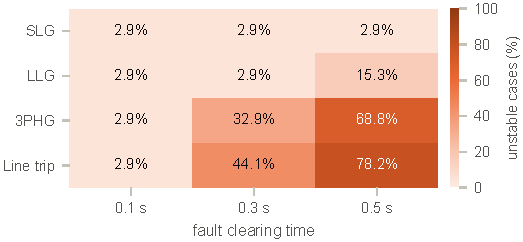
\includegraphics[width=\columnwidth]{fig_fault_time.pdf}
\caption{Share of unstable cases by fault type and fault clearing time.}
\label{fig:faulttime}
\end{figure}

\begin{figure}[t]
\centering
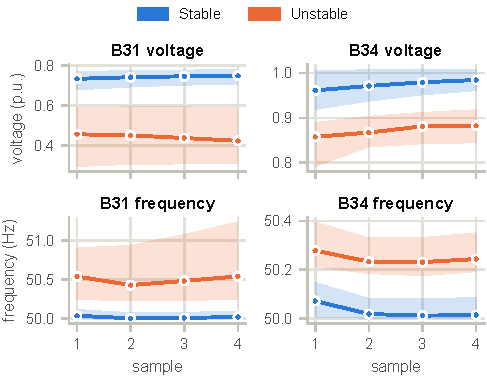
\includegraphics[width=\columnwidth]{fig_traces.pdf}
\caption{Median (line) and interquartile range (band) of the voltage and frequency at B31 and B34 over the four
samples, for stable and unstable cases.}
\label{fig:traces}
\end{figure}

%=====================================================================
\section{Methodology}
\label{sec:method}
%=====================================================================
The workflow is summarized in Fig.~\ref{fig:workflow}.

\begin{figure}[t]
\centering
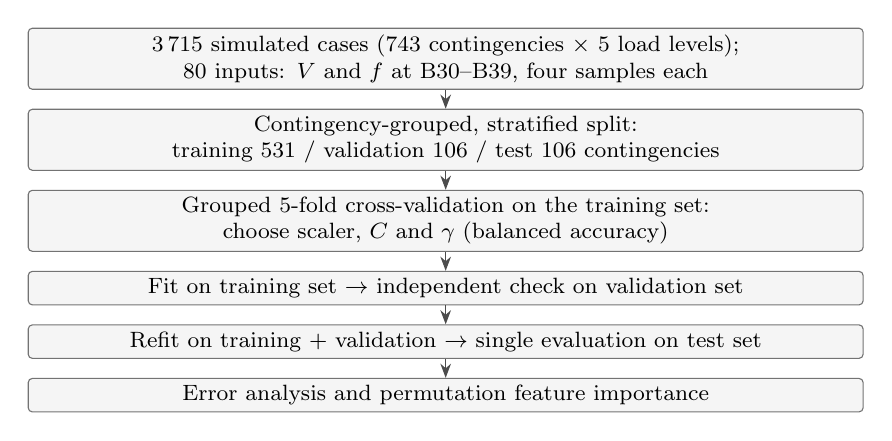
\begin{tikzpicture}[node distance=2.4mm,
  box/.style={draw=black!55, rounded corners=1.5pt, fill=black!4, align=center,
              text width=0.86\columnwidth, inner sep=2.5pt, font=\footnotesize},
  arr/.style={-{Stealth[length=1.8mm]}, black!70}]
  \node[box] (a) {3\,715 simulated cases (743 contingencies $\times$ 5 load levels);\\
                  80 inputs: $V$ and $f$ at B30--B39, four samples each};
  \node[box, below=of a] (b) {Contingency-grouped, stratified split:\\
                  training 531 / validation 106 / test 106 contingencies};
  \node[box, below=of b] (c) {Grouped 5-fold cross-validation on the training set:\\
                  choose scaler, $C$ and $\gamma$ (balanced accuracy)};
  \node[box, below=of c] (d) {Fit on training set $\rightarrow$ independent check on validation set};
  \node[box, below=of d] (e) {Refit on training + validation $\rightarrow$ single evaluation on test set};
  \node[box, below=of e] (f) {Error analysis and permutation feature importance};
  \draw[arr] (a) -- (b); \draw[arr] (b) -- (c); \draw[arr] (c) -- (d);
  \draw[arr] (d) -- (e); \draw[arr] (e) -- (f);
\end{tikzpicture}
\caption{Workflow of the proposed assessment.}
\label{fig:workflow}
\end{figure}

\subsection{Contingency-Grouped Data Split}
Because each contingency appears at five load levels with very similar responses, the data are split by contingency:
all variants of a contingency belong to the same subset. A stratified group split keeps the unstable share equal in
the training, validation and test sets (Table~\ref{tab:split}). The two contingencies containing the impossible
readings are assigned to the training set, so that the model is trained with them and later studies that remove or
cap them can be compared on identical validation and test sets.

\begin{table}[t]
\caption{Training, validation and test sets}
\label{tab:split}
\centering
\begin{tabular}{lrrrr}
\toprule
Set & Cases & Contingencies & Unstable & Unstable (\%) \\
\midrule
Training   & 2\,655 & 531 & 483 & 18.2 \\
Validation & 530    & 106 & 96  & 18.1 \\
Test       & 530    & 106 & 97  & 18.3 \\
\bottomrule
\end{tabular}
\end{table}

\subsection{Support Vector Machine}
With training pairs $(\mathbf{x}_i, y_i)$, $y_i = +1$ for stable and $-1$ for unstable cases, the soft-margin SVM
solves
\begin{equation}
\begin{aligned}
  &\min_{\mathbf{w}, b, \boldsymbol{\xi}} \; \tfrac{1}{2}\lVert\mathbf{w}\rVert^2 + C\sum_i c_{y_i}\xi_i \\
  &\;\text{s.t.} \;\; y_i\bigl(\mathbf{w}^\top\phi(\mathbf{x}_i) + b\bigr) \ge 1 - \xi_i,\;\; \xi_i \ge 0,
\end{aligned}
\end{equation}
with the radial basis function (RBF) kernel
$K(\mathbf{x}, \mathbf{x}') = \exp(-\gamma\lVert\mathbf{x} - \mathbf{x}'\rVert^2)$.
The class weights $c_k = n/(2n_k)$ compensate for the class imbalance; in the training set an error on an unstable
case costs about 4.5 times more than one on a stable case. The decision function is
\begin{equation}
  f(\mathbf{x}) = \sum_{i \in \mathrm{SV}} \alpha_i y_i K(\mathbf{x}_i, \mathbf{x}) + b,
\end{equation}
and we use the instability score $s(\mathbf{x}) = -f(\mathbf{x})$: a case is classified unstable if $s > 0$, and
$|s|$ indicates the distance from the decision boundary.

\subsection{Preprocessing and Hyperparameter Selection}
Two scalers were compared, both fitted on training data only: standardization
$z_j = (x_j - \mu_j)/\sigma_j$, and robust scaling
$z_j = \mathrm{clip}\bigl((x_j - \mathrm{med}_j)/\mathrm{IQR}_j, -20, 20\bigr)$, whose median and interquartile range
are insensitive to the impossible readings and whose clipping limits their influence on the kernel distance.
The grid $C \in \{0.1, 1, 10, 100, 1000\}$ and $\gamma \in \{1/(80\,\mathrm{Var}(\mathbf{z})), 0.001, 0.003, 0.01,
0.03, 0.1\}$ was evaluated for both scalers (60 combinations) by grouped five-fold cross-validation within the
training set, i.e., each fold holds out one fifth of the training contingencies. The setting with the highest mean
balanced accuracy was selected~\cite{hsu2003}. A single validation set is not used for this choice because, with
106 contingencies, its score is too noisy: the setting it favors ($C = 1000$, $\gamma = 0.03$, validation balanced
accuracy 0.993) reaches only 0.967 in cross-validation. The validation set instead serves as an independent check
before the test set is used once. The implementation uses scikit-learn~\cite{pedregosa2011}.

\subsection{Performance Metrics}
The unstable class is treated as positive. With TP, FN, FP and TN the counts of the confusion matrix,
\begin{equation}
  \mathrm{BA} = \frac{1}{2}\left(\frac{TP}{TP + FN} + \frac{TN}{TN + FP}\right),
\end{equation}
where $TP/(TP + FN)$ is the unstable recall (detection rate) and $TN/(TN + FP)$ the stable recall. Balanced accuracy
(BA) is used instead of accuracy because a classifier that always predicts ``stable'' would already be 81.8\,\%
accurate. The unstable precision $TP/(TP + FP)$ and the area under the ROC curve (AUC) complete the evaluation.

%=====================================================================
\section{Results}
\label{sec:results}
%=====================================================================
\subsection{Model Selection}
Cross-validation selects robust scaling with $C = 10$ and $\gamma = 0.001$, with a balanced accuracy of
$0.974 \pm 0.016$ (Fig.~\ref{fig:cvgrid}). The best standardized setting ($C = 100$, $\gamma = 0.001$) reaches
$0.972 \pm 0.013$, so the two scalers differ by less than the fold-to-fold spread. Small $C$ underfits
(0.91--0.94 at $C = 0.1$), and large $\gamma$ also degrades the result.

\begin{figure}[t]
\centering
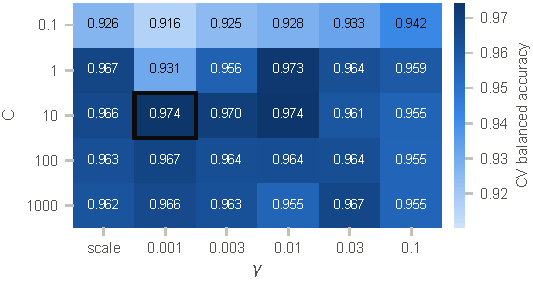
\includegraphics[width=\columnwidth]{fig_cv_grid.pdf}
\caption{Cross-validated balanced accuracy of the RBF SVM with robust scaling; the frame marks the selected setting.}
\label{fig:cvgrid}
\end{figure}

\subsection{Classification Performance}
Table~\ref{tab:results} summarizes the performance. Fitted on the training set, the model reaches BA = 0.961 on the
validation set, detecting 91 of 96 unstable cases with 11 false alarms. The final model, refitted on training and
validation data (3\,185 cases), reaches BA = 0.955 on the test set: it detects 93 of 97 unstable cases (95.9\,\%) and
raises 21 false alarms among 433 stable cases (Fig.~\ref{fig:confusion}). The ROC curves (Fig.~\ref{fig:roc}) confirm
that the instability score ranks unstable above stable cases very well (AUC of 0.994 on validation and 0.992 on
test). On the test set, load disconnections are classified without error, ground faults with 97.2\,\% and line trips
with 90.0\,\% accuracy, and the accuracy lies between 94.3\,\% and 97.2\,\% at every load level.

A learning curve on the validation set shows the BA rising from 0.87--0.92 with up to 1\,060 training cases to
0.96--0.97 with 1\,600 cases or more, after which it levels off.

\begin{table}[t]
\caption{Classification performance of the selected SVM}
\label{tab:results}
\centering
\setlength{\tabcolsep}{3.5pt}
\begin{tabular}{lccccc}
\toprule
Set & BA & \shortstack{Unstable\\recall} & \shortstack{Unstable\\precision} & \shortstack{Stable\\recall} & AUC \\
\midrule
Grouped CV       & 0.974$\pm$0.016 & -- & -- & -- & -- \\
Training         & 0.982 & 0.990 & 0.894 & 0.974 & 0.998 \\
Validation       & 0.961 & 0.948 & 0.892 & 0.975 & 0.994 \\
Test             & \textbf{0.955} & \textbf{0.959} & \textbf{0.816} & \textbf{0.952} & \textbf{0.992} \\
\bottomrule
\multicolumn{6}{l}{\footnotesize Training/validation: model fitted on the training set. Test: final model.}
\end{tabular}
\end{table}

\begin{figure}[t]
\centering
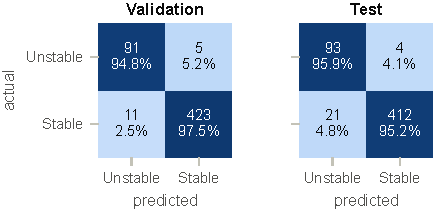
\includegraphics[width=\columnwidth]{fig_confusion.pdf}
\caption{Confusion matrices on the validation and test sets (count and share of each actual class).}
\label{fig:confusion}
\end{figure}

\begin{figure}[t]
\centering
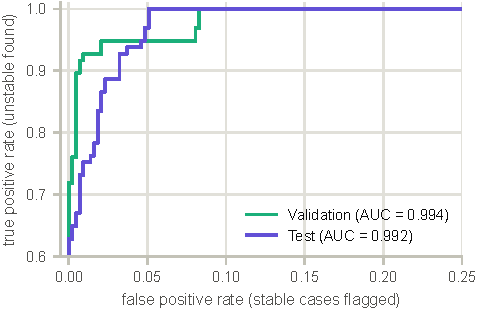
\includegraphics[width=\columnwidth]{fig_roc.pdf}
\caption{ROC curves on the validation and test sets (unstable as positive class), zoomed to the upper-left corner.}
\label{fig:roc}
\end{figure}

\subsection{Error Analysis}
The 25 test errors stem from only 13 contingencies, since a contingency that is difficult for the model tends to be
difficult at several load levels. Ten of the 21 false alarms come from two contingencies, each misclassified at all
five load levels. The first is the trip of the generator at bus~38: after this trip the B38 frequency falls as low as
49.92\,Hz, below every training case (minimum 49.977\,Hz), so the SVM extrapolates outside the region covered by its
support vectors. Overall, 32 test cases have at least one input outside the training range; five of them are
misclassified, all belonging to this contingency. The second is the 0.3-s trip of line 22--23, which the model flags
with high confidence ($s = 1.3$--$2.3$), indicating that its early response resembles that of unstable cases. The
remaining false alarms are LLG and 3PHG faults and line trips cleared after 0.3--0.5\,s, i.e., severe but
survivable disturbances near the stability boundary. The four missed unstable cases (3PHG faults on lines 28--29 and
21--22 and an LLG fault on line 4--5) all lie just below the boundary ($-0.15 \le s \le -0.05$). On the validation
set, the five missed cases are all variants of a 0.1-s 3PHG fault on line 16--19: the short fault leaves only small
deviations in the four samples, although the subsequent loss of the line is always unstable.

\subsection{Feature Importance}
Permutation importance, computed by jointly shuffling the four samples of one quantity at one bus over the test
cases, is shown in Fig.~\ref{fig:importance}. The model relies most on the B31 voltage and the B34 frequency
(balanced-accuracy drops of 0.121 and 0.119), followed by the B38 voltage (0.050) and the B31 frequency (0.032). This
agrees with the physics of the dataset: B31 exhibits the deepest voltage depression in unstable cases, and B34 is one
of the two generators separated by the loss of line 16--19. Several inputs, e.g., the B30 voltage and frequency, add
no information once the others are known.

\begin{figure}[t]
\centering
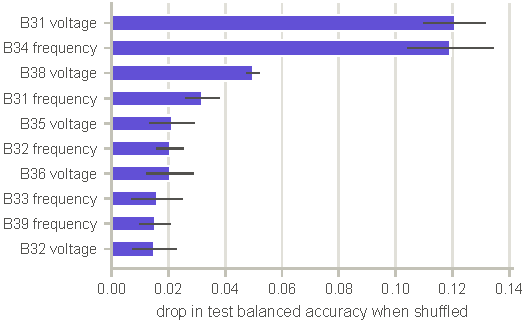
\includegraphics[width=\columnwidth]{fig_importance.pdf}
\caption{Permutation importance of the ten most important bus quantities (mean $\pm$ standard deviation over ten
repetitions).}
\label{fig:importance}
\end{figure}

%=====================================================================
\section{Discussion}
\label{sec:discussion}
%=====================================================================
The three performance estimates (cross-validation 0.974, validation 0.961, test 0.955) differ by up to two points
because each hold-out set contains only about 106 contingencies and the errors cluster in a few of them; the test set
happens to contain the two contingencies responsible for ten false alarms. A realistic expectation for unseen
contingencies of the simulated families is therefore a balanced accuracy of about 0.95--0.97. These figures refer to
contingencies never seen during training; a random split of the cases would place near-identical variants of each
test contingency in the training set and produce higher but misleading scores.

Most errors are false alarms, which is the safer direction for operation. The systematic errors arise where the
measurements leave the range covered by the training data, as for the bus-38 generator trip, which is one of only
nine generator-trip contingencies available for training. Reporting inputs outside the training range together with
each prediction is a simple safeguard. The impossible readings were retained in this study; with them in the training
data, robust scaling was marginally preferred over standardization. Limitations are the use of simulated data of a
single test system, the small number of generator-trip scenarios, and the short observation window of four samples,
in which slowly developing instability leaves little trace.

%=====================================================================
\section{Conclusion}
\label{sec:conclusion}
%=====================================================================
An RBF-kernel SVM using only four voltage and four frequency samples from each generator bus predicts the transient
stability of the IEEE 39-bus system with a balanced accuracy of 0.955 on unseen contingencies, detecting 95.9\,\% of
the unstable cases with an AUC of 0.992. A contingency-grouped split and grouped cross-validation are essential for
an honest estimate. Future work will examine the removal or capping of the impossible readings, extend the scenario
set, in particular with generator trips, tune the decision threshold to trade false alarms against missed unstable
cases, and add engineered features such as the frequency spread between generators.

% TODO: verify the details of every reference before submission
\begin{thebibliography}{00}
\bibitem{kundur2004definition} P. Kundur \textit{et al.}, ``Definition and classification of power system
stability,'' \textit{IEEE Trans. Power Syst.}, vol.~19, no.~3, pp.~1387--1401, Aug. 2004.
\bibitem{kundur1994} P. Kundur, \textit{Power System Stability and Control}. New York, NY, USA: McGraw-Hill, 1994.
\bibitem{cortes1995} C. Cortes and V. Vapnik, ``Support-vector networks,'' \textit{Mach. Learn.}, vol.~20, no.~3,
pp.~273--297, 1995.
\bibitem{scholkopf2002} B. Sch{\"o}lkopf and A. J. Smola, \textit{Learning with Kernels}. Cambridge, MA, USA: MIT
Press, 2002.
\bibitem{moulin2004} L. S. Moulin, A. P. Alves da Silva, M. A. El-Sharkawi, and R. J. Marks II, ``Support vector
machines for transient stability analysis of large-scale power systems,'' \textit{IEEE Trans. Power Syst.}, vol.~19,
no.~2, pp.~818--825, May 2004.
\bibitem{gomez2011} F. R. Gomez, A. D. Rajapakse, U. D. Annakkage, and I. T. Fernando, ``Support vector
machine-based algorithm for post-fault transient stability status prediction using synchronized measurements,''
\textit{IEEE Trans. Power Syst.}, vol.~26, no.~3, pp.~1474--1483, Aug. 2011.
\bibitem{athay1979} T. Athay, R. Podmore, and S. Virmani, ``A practical method for the direct analysis of transient
stability,'' \textit{IEEE Trans. Power App. Syst.}, vol.~PAS-98, no.~2, pp.~573--584, Mar. 1979.
\bibitem{xu2012} Y. Xu, Z. Y. Dong, J. H. Zhao, P. Zhang, and K. P. Wong, ``A reliable intelligent system for
real-time dynamic security assessment of power systems,'' \textit{IEEE Trans. Power Syst.}, vol.~27, no.~3,
pp.~1253--1263, Aug. 2012.
\bibitem{hsu2003} C.-W. Hsu, C.-C. Chang, and C.-J. Lin, ``A practical guide to support vector classification,''
Dept. Comput. Sci., Nat. Taiwan Univ., Taipei, Taiwan, Tech. Rep., 2003.
\bibitem{pedregosa2011} F. Pedregosa \textit{et al.}, ``Scikit-learn: Machine learning in Python,'' \textit{J. Mach.
Learn. Res.}, vol.~12, pp.~2825--2830, 2011.
\end{thebibliography}

\end{document}
